This was seen on the
\href{https://data.ohio.gov/wps/portal/gov/data/view/covid-19-reporting}{data
dashboard}:

\begin{figure}
\centering
\pandocbounded{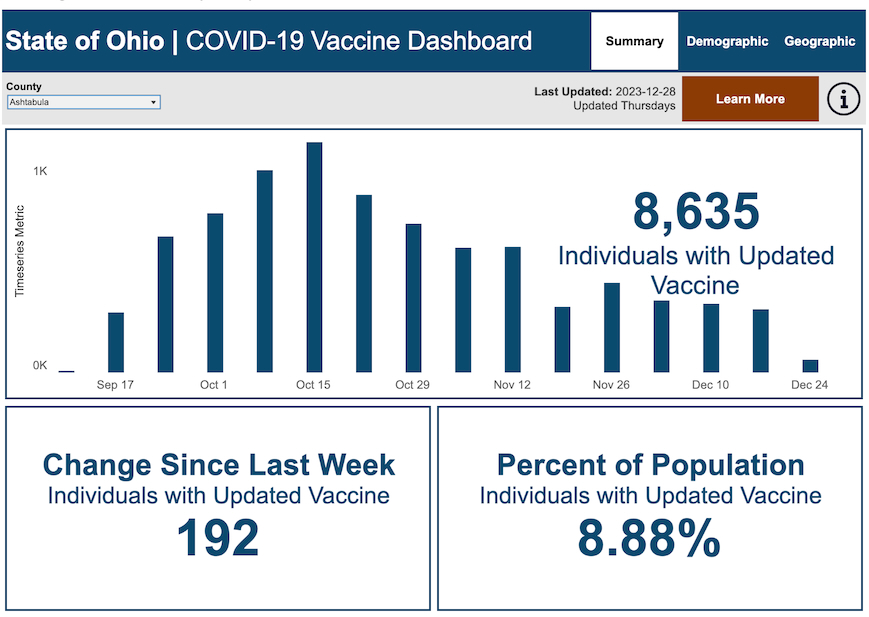
\includegraphics[keepaspectratio]{\%7B\%7Bsite.url\%7D\%7D/img/vaxing-end-of-2023.jpg}}
\caption{Dashboard screenshot showing only 8,635 residents of Ashtabula
County have received the updated COVID-19 vaccine. That is only 8.88\%
of the local population! This is not good.}
\end{figure}

I am just at a loss. This is just another facet of our
\href{https://www.countyhealthrankings.org/explore-health-rankings/ohio/ashtabula?year=2023}{poor
health outcomes locally}. It isn't like
\href{https://www.cdc.gov/places/index.html}{PLACES} shows Ashtabula
County in all that great of a shape.

I have to assess options.
